Figure~\ref{fig:4:fw} in Chapter~\ref{chap:cc.fw} shows the structure of the
congestion control framework described in this thesis. The framework
categorizes \emph{In-path} sources and \emph{In-band} signaling for
implementing congestion control (corresponds to \emph{Block A} in
Figure~\ref{fig:4:fw}), which are discussed in this chapter. This chapter is
based on our work on congestion control for interactive multimedia
applications, which is documented in \citepub{c:3grc}, \citepub{c:hetrc},
\citepub{c:eval}, \cite{draft.xr.discard.rle},
\cite{draft.xr.bytes.discarded}, \cite{singh:2010.thesis} and
\cite{Singh:control.loops.api}.

In \citepub{c:3grc}, we propose a new congestion control algorithm for the
mobile (e.g., 3G) environment, to be deployed in IP Multimedia System (IMS).
The main distinction between mobile (e.g., 3G, LTE) and other wireless
environments (e.g., 802.11x) is the media streams are transmitted using the
\emph{unacknowledged mode}; the packets corrupted due to bit-errors (e.g.,
wireless interference) are not re-transmitted. Hence, the packets incur low
delay, compared to Wireless LAN where corrupted packets are retransmitted by
the link layer. We evaluate the performance of a sender-driven congestion
control with a receiver-driven congestion control and evaluate the performance
of the proposed congestion control algorithm in a simulated environment (in
ns-2) using real-world 3G traces~\cite{s4.eval.bitrate, 3gppSim}. In
\citepub{c:hetrc}, we extend the approach in \citepub{c:3grc} for deploying on
the Internet and show that the congestion control scheme is deployable. In
\cite{draft.xr.discard.rle} and \cite{draft.xr.bytes.discarded}, we propose
RTCP XR block extensions that indicate the number of bytes discarded and
run-length encoding of discarded packets, respectively. These packets are
discarded by the receiver because they arrived too early or too late to be
played out by the receiver. This information is used as a congestion cue by
the sender.

\cite{Singh:control.loops.api} discusses the application and API requirements
for interactive multimedia congestion control. It describes the two control
loops: a) between the receiver and the sender, and b) between the media
encoder and the sending agent. In the first loop, the receiver notifies the
sender about the current network characteristics. In the second loop, the
sending agent requests a new media bit rate, and the encoder tries at best to
meet it, sometimes under-shooting or over-shooting the requested rate.

Lastly, in \citepub{c:eval} we evaluate the performance of a congestion
control algorithm proposed by Google for WebRTC. We evaluate the performance
in diverse scenarios measuring scalability (\emph{how quickly is the
congestion control able to utilize the available capacity}), self-fairness and
competing against bursty cross-traffic. We evaluate the performance of
web-browsers implementing the congestion control algorithm in our testbed that
emulates the diverse scenarios.

\section{Schemes of Congestion Control}

\begin{figure}
  \centerline{
    \subfloat[Sender-driven Scheme]{
      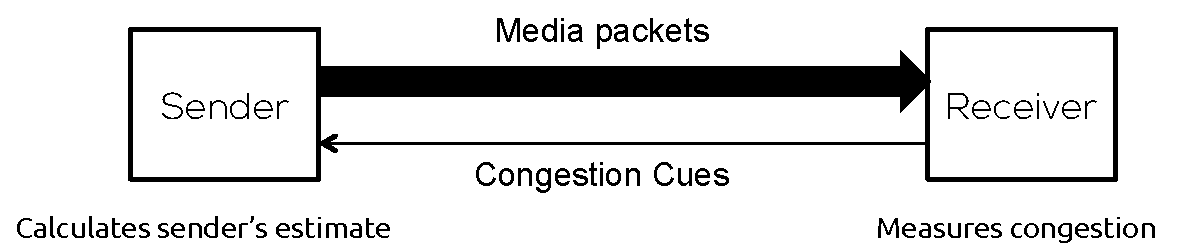
\includegraphics[width=0.9\textwidth]
      {chap5-fig-cc-scheme-s}
    }
  }
  \centerline{
    \subfloat[Receiver-driven Scheme]{
      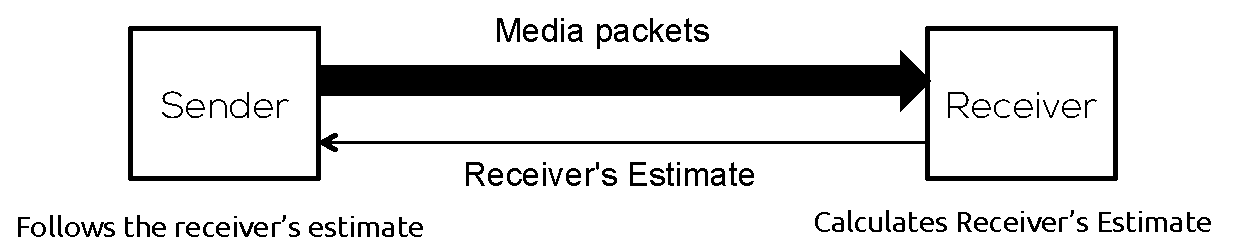
\includegraphics[width=0.9\textwidth]
      {chap5-fig-cc-scheme-r}
    }
  }
  \centerline{
    \subfloat[Co-operative Scheme]{
      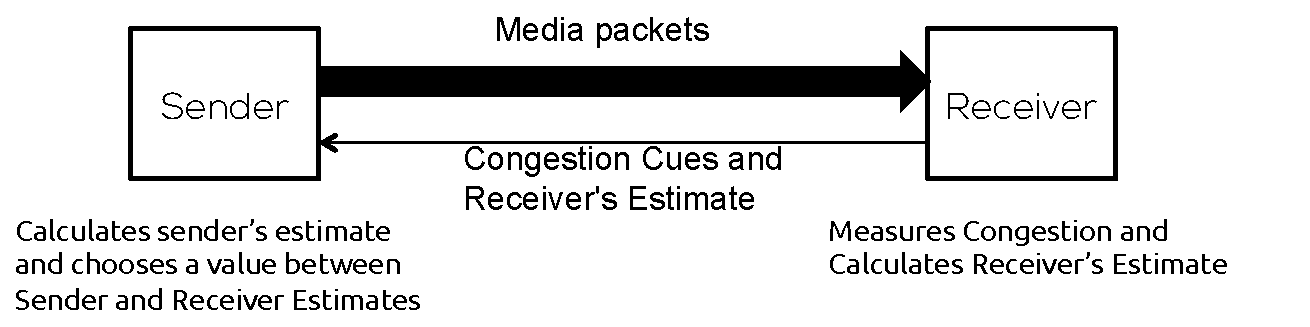
\includegraphics[width=0.9\textwidth]
      {chap5-fig-cc-scheme-c}
    }
  }
  \caption{Congestion control schemes a) sender-driven, b) receiver-driven
and c) co-operative.}
  \label{fig:cc:scheme}
\end{figure}

The congestion control algorithm can be implemented at the sender, at the
receiver, or the sender and receiver operate co-operatively. The
\emph{sender-driven} scheme requires that the receiver measure the current
network condition and signal the observed congestion cues to the sender, which
calculates the sender's estimate and uses it as the new sending rate. In the
\emph{receiver-driven} scheme, the receiver calculates the new sending rate
(receiver's estimate) based on the observed congestion cues, and signals the
new rate to the sender, which on receiving the new rate, adapts the media bit
rate to received value. The \emph{co-operative} scheme is an extension to the
\emph{sender-driven} scheme, in this case, the receiver calculates the
receiver's estimated rate and signals it along with the observed congestion
cues, the sender at its end calculates the sender's estimate based on the
congestion cues and chooses a new sending rate, typically, between the
sender's estimate and the receiver's estimate. Figure~\ref{fig:cc:scheme}
shows the interaction of the sender and receiver for each scheme. The figure
merely shows the media flow in one direction, however, it should be noted that
the media in the simulation and the emulated testbed actually flow in both
directions unless explicitly mentioned. This is mainly done for the
convenience of representation and followed throughout the remainder of the
thesis.



\section{Sender-driven Congestion Control Schemes}

TCP Friendly Rate Control (TFRC) is an equation based congestion control
algorithm implemented at the sender~\cite{tfrc_347397} and is also implemented
as a profile~\cite{rfc4342} in the Datagram Congestion Control Protocol
(DCCP)~\cite{rfc4340}. TFRC uses the average packet size, RTT,
loss-rate~\cite{rfc3448} to calculate the new sending rate.
\cite{draft.rtp.tfrc} maps the timing rules defined in~\cite{rfc4828, rfc5348}
to that of RTP/RTCP feedback loop, it also redefines the timing rules in
AVPF-profile~\cite{rfc4585} for very short RTTs ($<20ms$).
\cite{Gharai06:ICME} shows that TFRC is stable on large RTT paths but less
stable for shorter paths~\cite{saurin:2006:thesis}. Our results in
\citepub{c:3grc} shows that TFRC underutilizes the link (average bandwidth
utilization (ABU) is between 30-40\%) and has higher fractional loss (\~6\%)
which results in lower PSNR. One disadvantage of TFRC is that it produces a
sawtooth sending rate \cite{saurin:2006:thesis}, \citepub{c:3grc}.
Figure~\ref{fig:tfrc} shows the performance of TFRC on a slow time-varying
link and a 3G link.

\begin{figure}
  \centerline{
    \subfloat{
      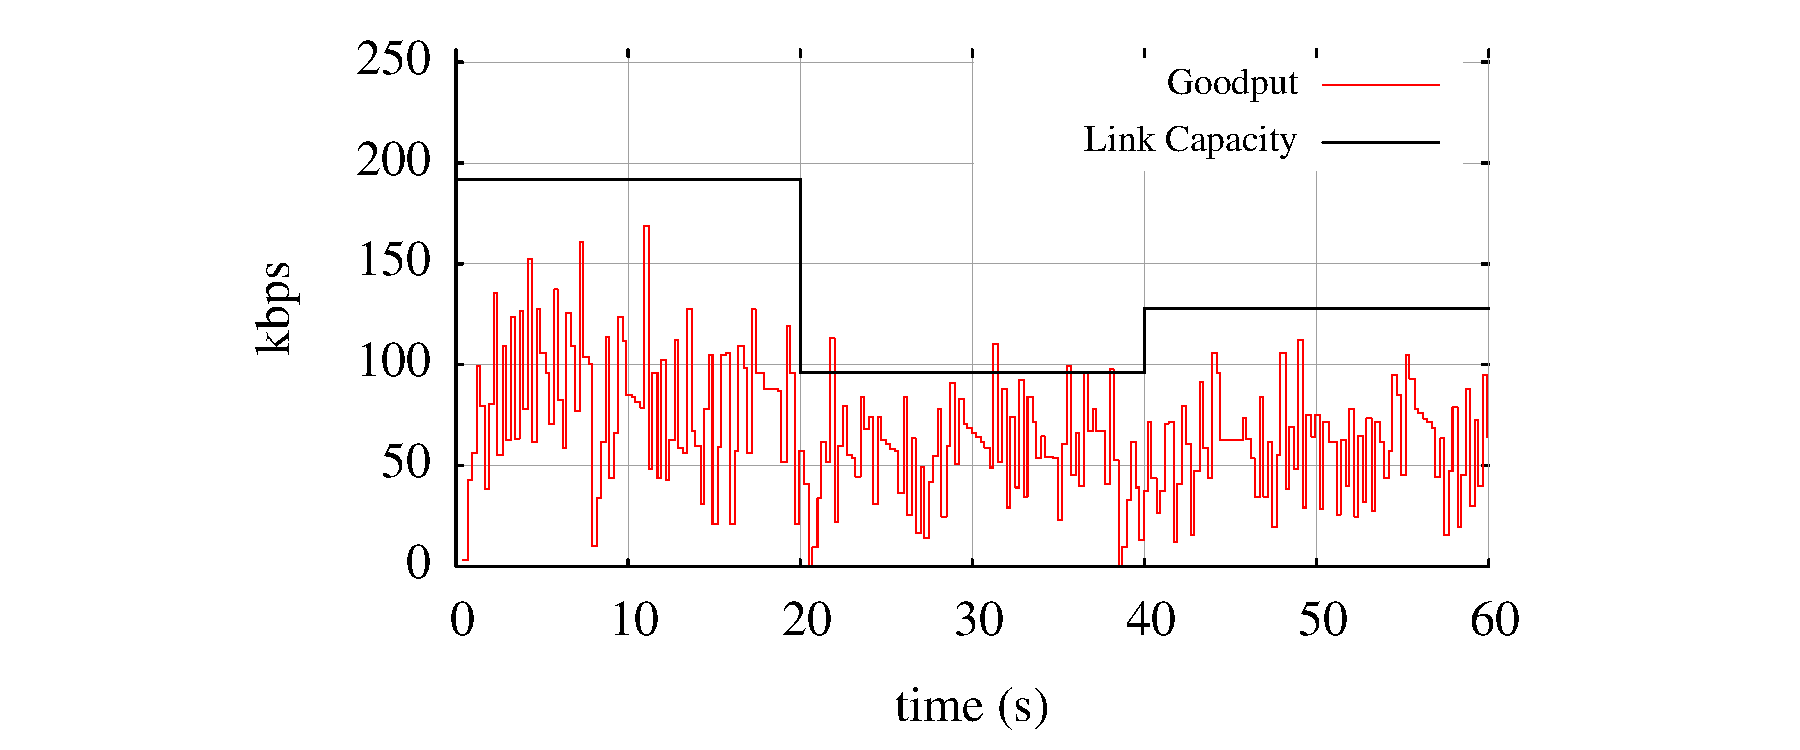
\includegraphics[width=0.5\textwidth, clip=true, trim=3cm 0 4.5cm 0]
      {chap5_graph_sl_tfrc}
    }
    \subfloat{
      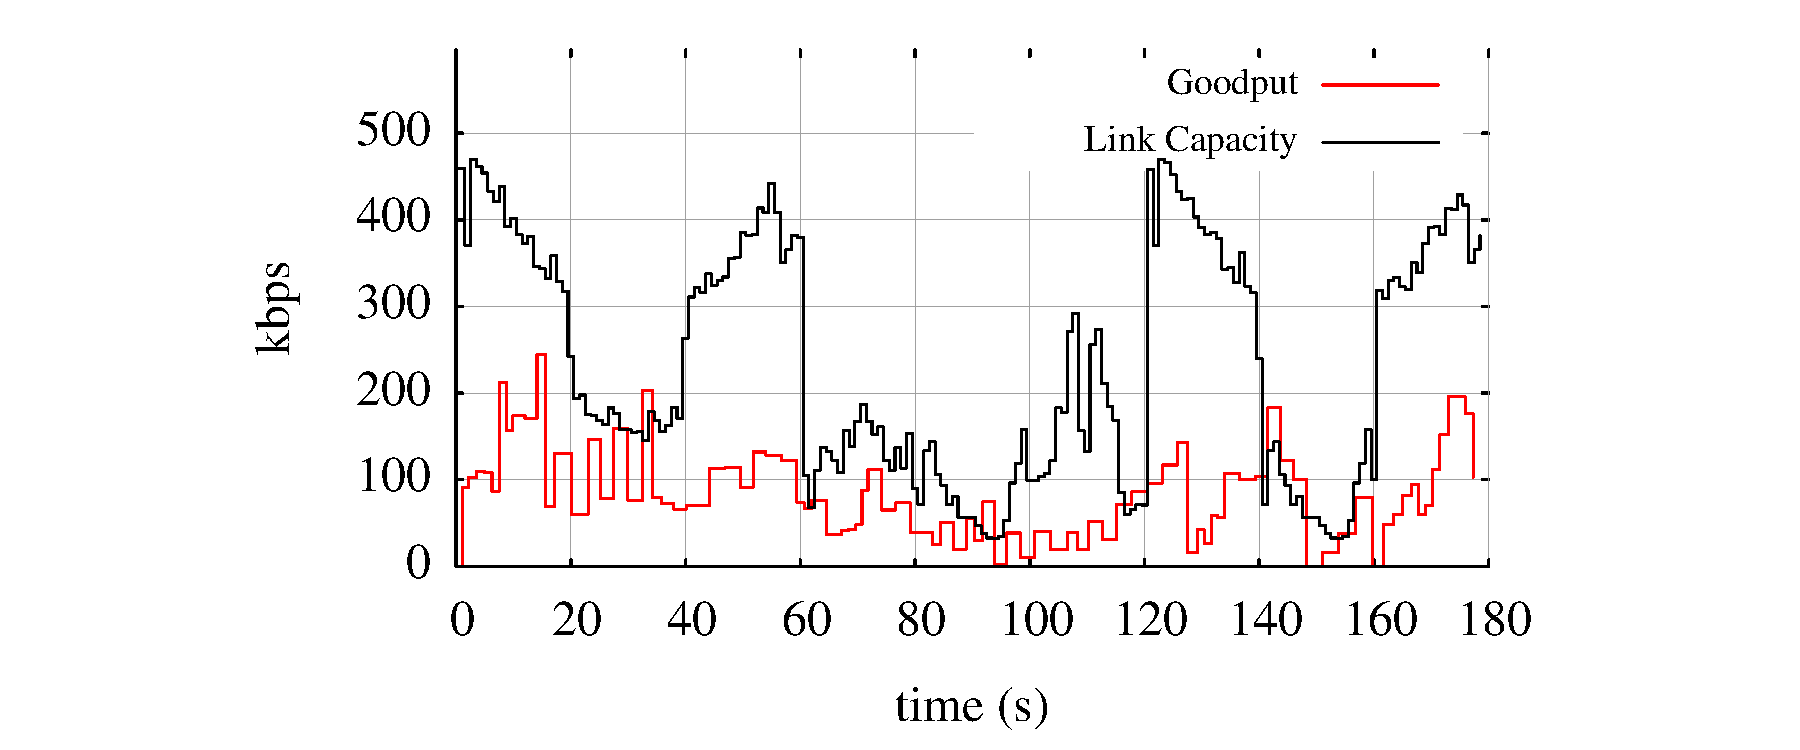
\includegraphics[width=0.5\textwidth, clip=true, trim=3cm 0 4.5cm 0]
      {chap5_graph_3g_tfrc_1}
    }
  }
  \caption{Performance of TFRC in a slow time-varying link and 3G network.}
  \label{fig:tfrc}
\end{figure}

Rate Adaption Protocol (RAP)~\cite{rap:752152} uses a windowed-approach and
this too exhibits a sawtooth-type of behavior. Any algorithm that consistently
produces a sawtooth media rate is not well suited for real-time communication
because it generates a poor user-experience
\cite{Gharai:2002wt,VladBalan:2007dq, Zink03subjectiveimpression}. Instead of
just relying on RTT and loss for congestion control, Garudadri~\textit{et
al.}~\cite{4397059} also use the receiver playout buffer to detect
underutilization and overuse, i.e., the receiver signals to the sender the
current receiver buffer occupancy. Zhu~\textit{et al.}~\cite{rmcat-nada} use
Pre-Congestion Notification (PCN), Explicit Congestion Notification (ECN) and
loss rate to get an accurate estimate delay estimate for implementing
congestion control. In this case, they assume all packets marked by ECN and
PCN as lost. O'Hanlon~\textit{et al.}~\cite{rmcat-dflow} propose using a
delay-based estimate when competing with similar traffic and using a
windowed-approach when competing with TCP-type cross traffic, they switch
modes by using a threshold on the observed end-to-end delay, the idea is
similar to the one discussed in~\cite{budzisz2011fair}.


\section{Receiver-driven Congestion Control Schemes}

Temporary Maximum Media Bit-rate Request (TMMBR) is defined as a codec control
messages in \cite{rfc5104}, it is generated by the receiver in a
point-to-point video call. The receiver calculates new estimate based on the
average inter-arrival time of RTP packets (\emph{video frames}) between two
RTCP RRs. The TMMBR indicates to the sender to limit its maximum sending rate
to the value requested in the message. 3GPP~\cite{3gpp.26.114} also uses TMMBR
messages to notify the sender of the expected sending rate. Our results in
\citepub{c:3grc} shows that TMMBR-based congestion control utilizes the link
better than TFRC (ABU between 50-70\%) and much lower fractional loss
($\le$2\%). Figure~\ref{fig:tmmbr} shows the performance of TMMBR on a slow
time-varying link and a 3G link.

\begin{figure}
  \centerline{
    \subfloat{
      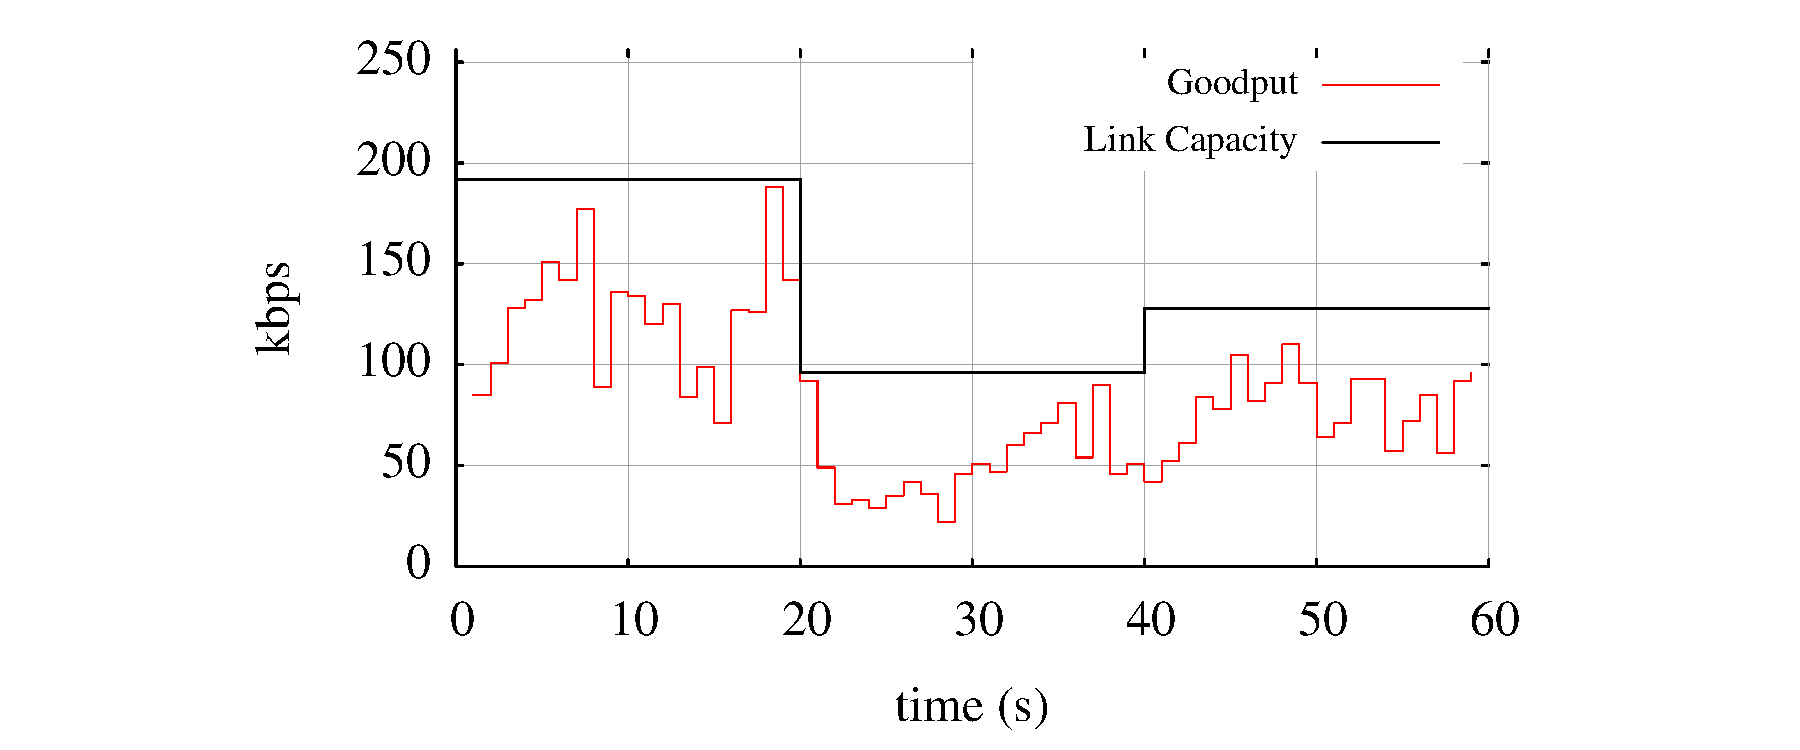
\includegraphics[width=0.5\textwidth, clip=true, trim=3cm 0 4.5cm 0]
      {chap5_graph_sl_tmmbr}
    }
    \subfloat{
      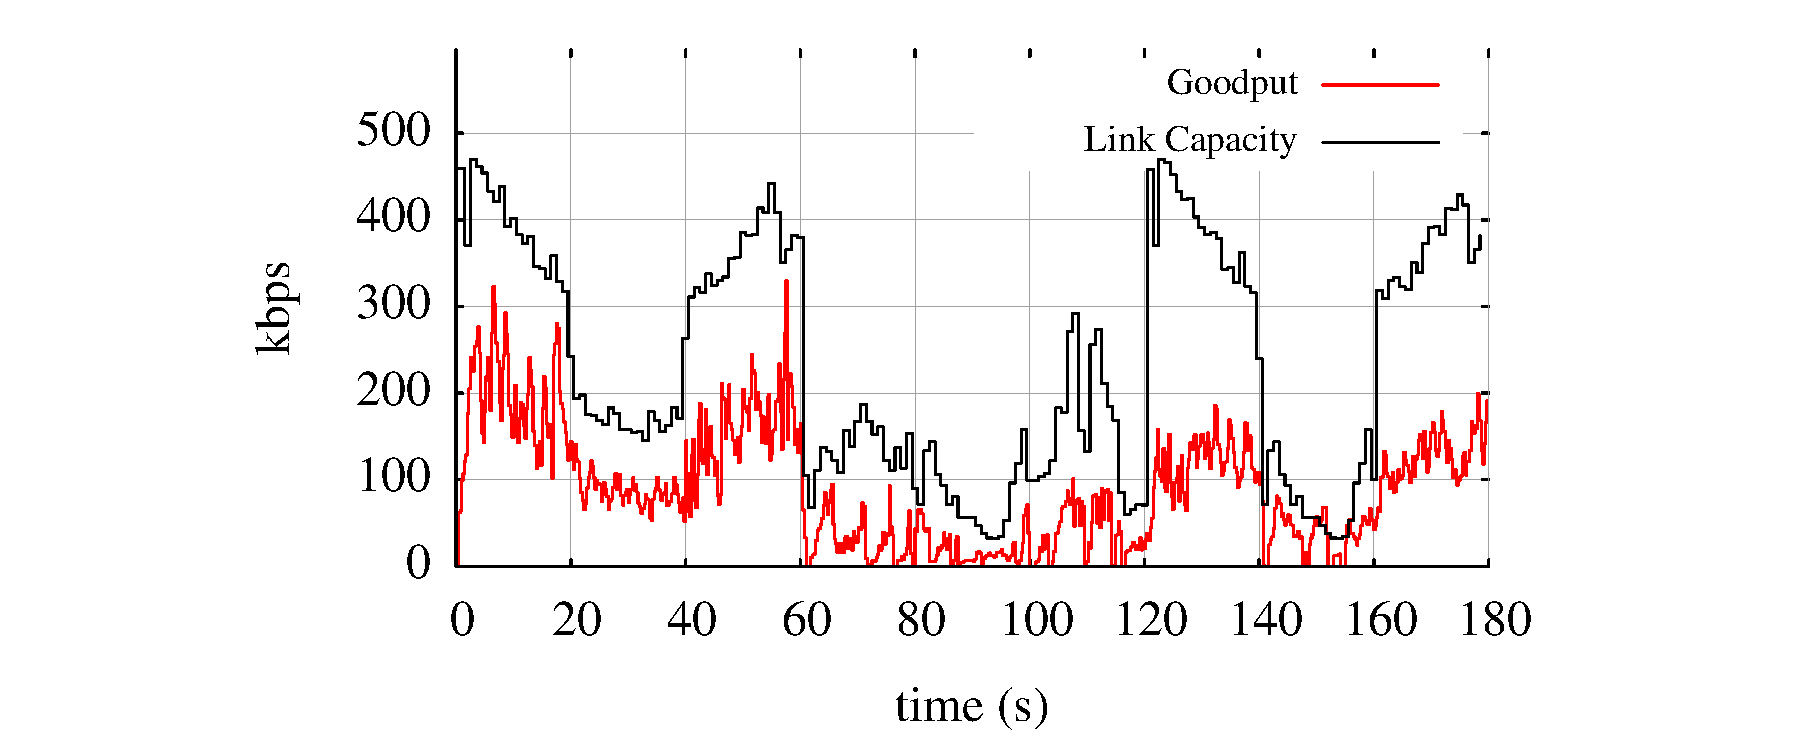
\includegraphics[width=0.5\textwidth, clip=true, trim=3cm 0 4.5cm 0]
      {chap5_graph_3g_tmmbr_u}
    }
  }
  \caption{Performance of TMMBR in a slow time-varying link and 3G network.}
  \label{fig:tmmbr}
\end{figure}

\section{Co-operative Congestion Control Schemes}
\label{cc:co-op}

Next Application Data Unit (NADU) signaling for video
streaming~\cite{nadu.1070341,nadu.1530486}. NADU is designed for rate
adaptation for video streaming in 3GPP~\cite{3gpp.26.234}. A NADU receiver
measures the playout delay (as a measure of buffer occupancy in time) and
signals it to the sender along with the next sequence number to be played out.
Conversational NADU (C-NADU) is an extension to NADU for congestion control
for interactive multimedia and is described in \citepub{c:3grc} and
\citepub{c:hetrc}. In C-NADU, the receiver also calculates the
\emph{receiver's capacity estimate} by measuring the frame inter-arrival time
and signals that along with the NADU report. If the video frame arrives at the
expected time, the receiver estimates no ongoing congestion, and if it arrives
later than the expected time, it is considered late and the receiver estimates
overuse. If the frame is delayed and misses its playout time, it is discarded
and in this case the receiver estimates congestion. Based on the above cases,
the receiver estimates the current capacity and signals it to the sender. At
the sender, the application calculates the TCP-friendly rate, and measures the
variation in RTT (75 and 90 percentile values) and if fraction of frames that
missed their playout deadline. In \citepub{c:3grc}, we show that C-NADU has
higher bandwidth utilization compared to TMMBR and TFRC.
Figure~\ref{fig:cnadu} shows the performance of C-NADU on a slow time-varying
link and a 3G link. Additionally, in \citepub{c:hetrc}, we show that C-NADU is
self-fair with other C-NADU flows in both wired and wireless
environments~\cite{singh:2010.thesis} and in \citepub{c:fecrc} we show that it
competes fairly with TCP cross-traffic, both long and short (bursty) TCP
flows.

\begin{figure}
  \centerline{
    \subfloat{
      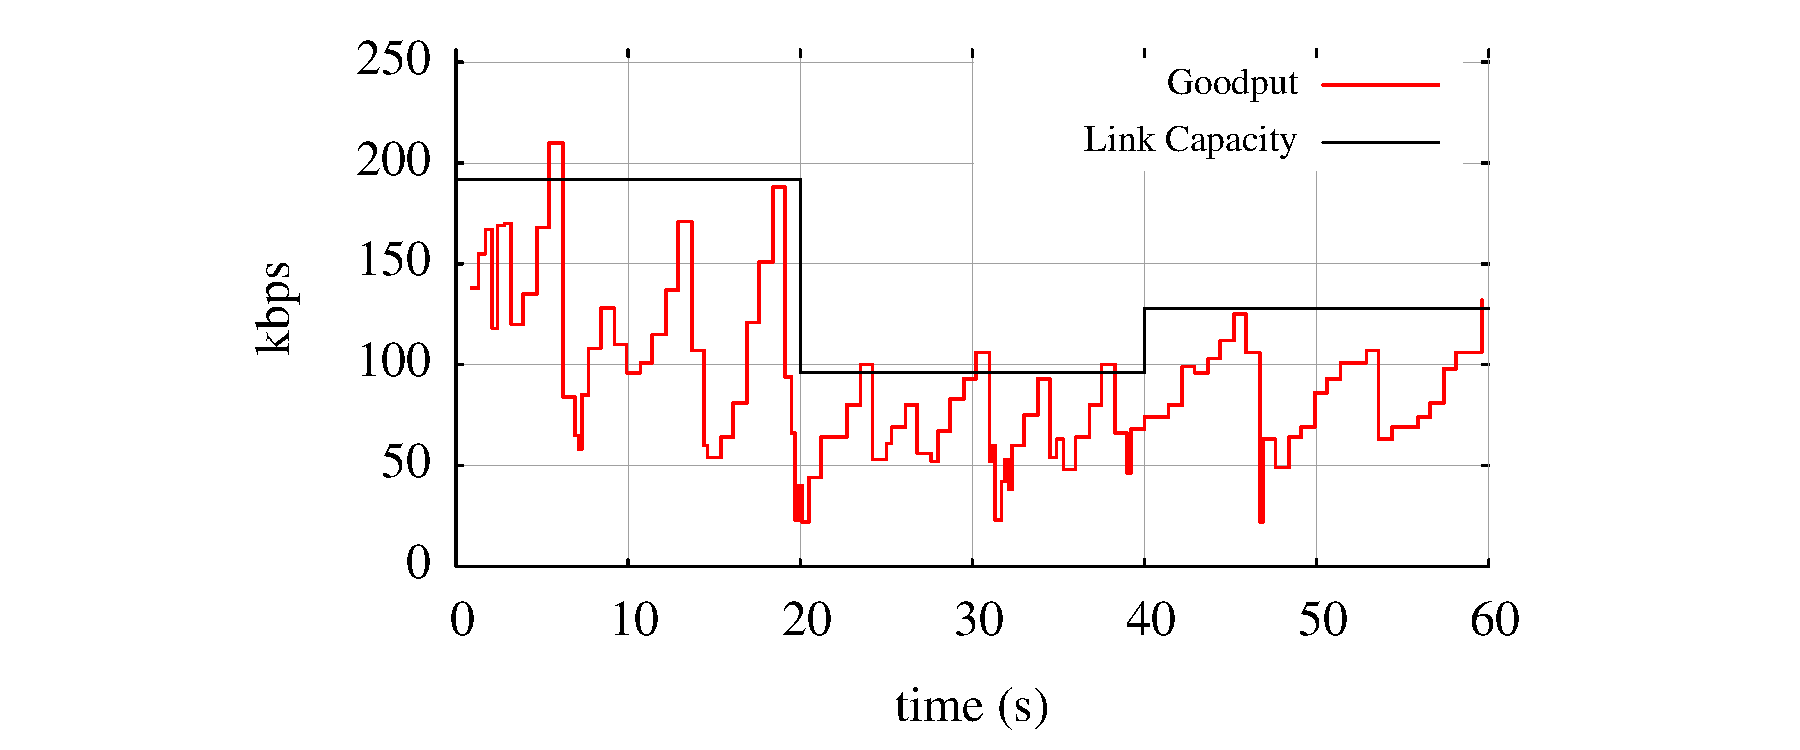
\includegraphics[width=0.5\textwidth, clip=true, trim=3cm 0 4.5cm 0]
      {chap5_graph_sl_cnadu}
    }
    \subfloat{
      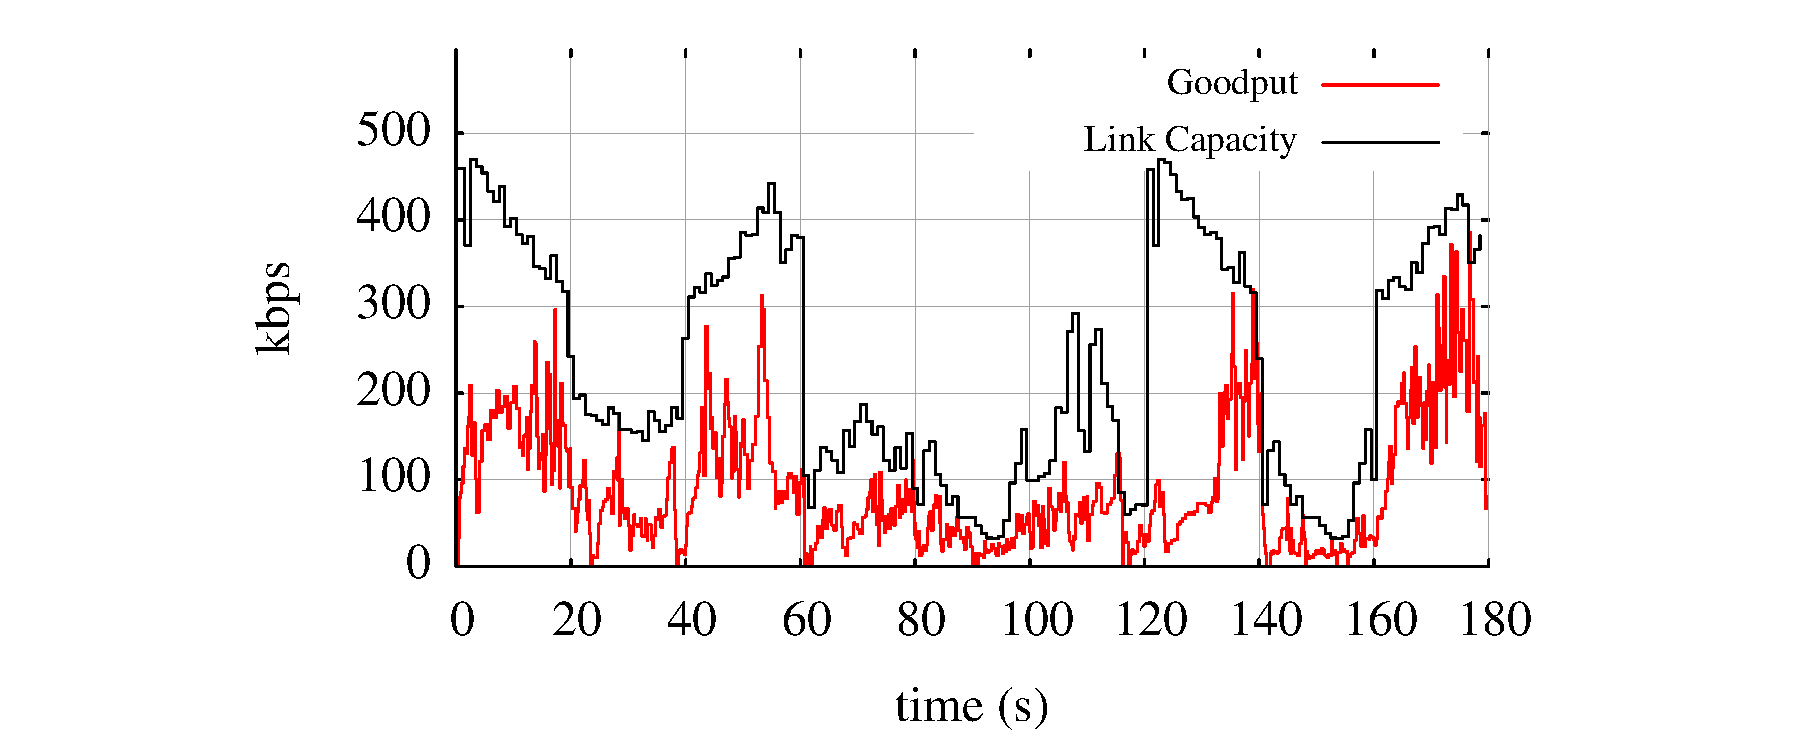
\includegraphics[width=0.5\textwidth, clip=true, trim=3cm 0 4.5cm 0]
      {chap5_graph_3g_cnadu}
    }
  }
  \caption{Performance of C-NADU in a slow time-varying link and 3G network.}
  \label{fig:cnadu}
\end{figure}

Receiver-side Real-Time Congestion Control (RRTCC) is described in
\cite{draft.rrtcc} and is proposed as one of the solution candidates for
WebRTC by Google. Like C-NADU, RRTCC also has a receiver- and sender-side
component. The receiver-side measures the capacity overuse and underuse by
monitoring the timestamp jitter of the incoming frames. The arrival-times are
modeled as a white Gaussian process; when the mean is 0 there is no
congestion, the mean is expected to increase when there is ongoing congestion
and expected to decrease when the congestion abates. Based on this
expectation, the receiver calculates the capacity estimate and signals it to
the sender. The sender calculates its estimate based on TFRC and finally,
chooses the new sending rate as a value between the TFRC rate calculated by
the sender and receiver estimate. Full details can be found in the
Internet-Draft~\cite{draft.rrtcc}. In \citepub{c:eval}, we evaluate the
performance of RRTCC in several scenarios: by itself on a bottleneck link,
competing with other RRTCC flows and competing with TCP cross-traffic.
Figure~\ref{fig:rrtcc} shows an example plot of the performance of RRTCC when
increasing latency and fractional loss. For example, in
Figure~\ref{fig:rrtcc}(a) by increasing the bottleneck link latency reduces
the sending rate of RRTCC.

\begin{figure}
  \centerline{
    \subfloat{
      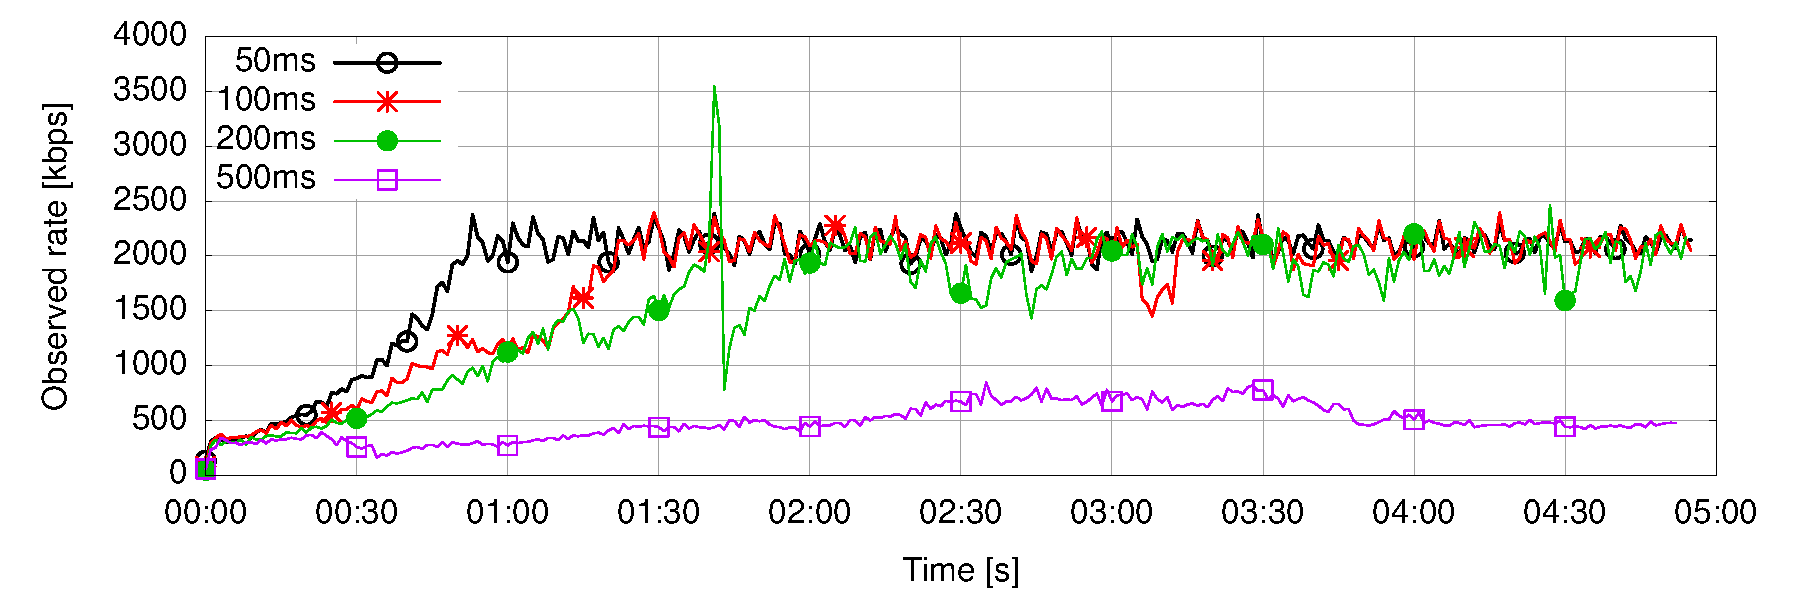
\includegraphics[width=0.7\textwidth]
      {chap5-graph-rrtcc-latency}
    }
   }
   \centerline{
    \subfloat{
      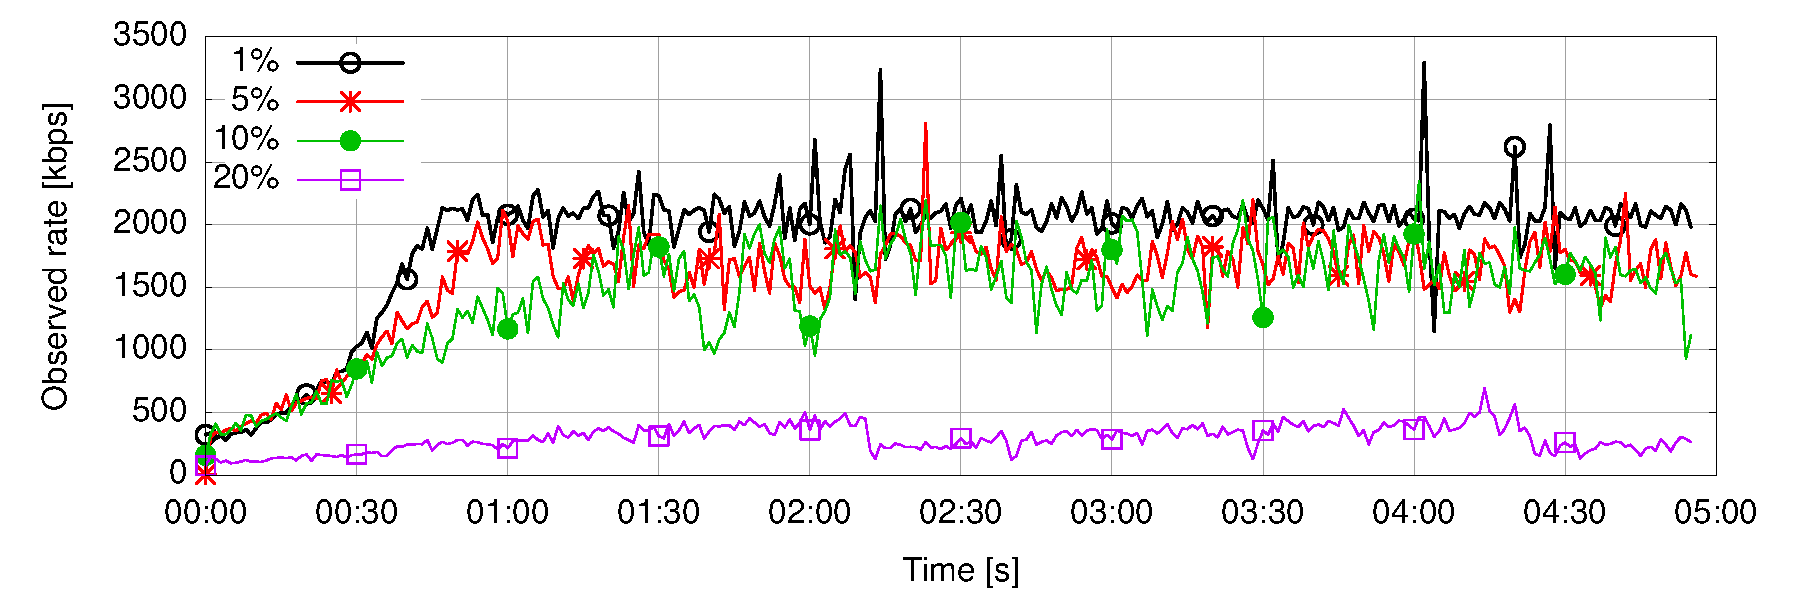
\includegraphics[width=0.7\textwidth]
      {chap5-graph-rrtcc-plr}
    }
  }
  \caption{Performance of RRTCC on a link with varying delay and fractional
  loss rate. We observe that by the sending rate decreases when increasing
  link latency or bit-error loss. }
  \label{fig:rrtcc}
\end{figure}

% \section{Summary}
% 
% In this section, we introduced 
